\documentclass[10pt,a4paper]{article}\usepackage[]{graphicx}\usepackage[]{color}
% maxwidth is the original width if it is less than linewidth
% otherwise use linewidth (to make sure the graphics do not exceed the margin)
\makeatletter
\def\maxwidth{ %
  \ifdim\Gin@nat@width>\linewidth
    \linewidth
  \else
    \Gin@nat@width
  \fi
}
\makeatother

\definecolor{fgcolor}{rgb}{0.345, 0.345, 0.345}
\newcommand{\hlnum}[1]{\textcolor[rgb]{0.686,0.059,0.569}{#1}}%
\newcommand{\hlstr}[1]{\textcolor[rgb]{0.192,0.494,0.8}{#1}}%
\newcommand{\hlcom}[1]{\textcolor[rgb]{0.678,0.584,0.686}{\textit{#1}}}%
\newcommand{\hlopt}[1]{\textcolor[rgb]{0,0,0}{#1}}%
\newcommand{\hlstd}[1]{\textcolor[rgb]{0.345,0.345,0.345}{#1}}%
\newcommand{\hlkwa}[1]{\textcolor[rgb]{0.161,0.373,0.58}{\textbf{#1}}}%
\newcommand{\hlkwb}[1]{\textcolor[rgb]{0.69,0.353,0.396}{#1}}%
\newcommand{\hlkwc}[1]{\textcolor[rgb]{0.333,0.667,0.333}{#1}}%
\newcommand{\hlkwd}[1]{\textcolor[rgb]{0.737,0.353,0.396}{\textbf{#1}}}%
\let\hlipl\hlkwb

\usepackage{framed}
\makeatletter
\newenvironment{kframe}{%
 \def\at@end@of@kframe{}%
 \ifinner\ifhmode%
  \def\at@end@of@kframe{\end{minipage}}%
  \begin{minipage}{\columnwidth}%
 \fi\fi%
 \def\FrameCommand##1{\hskip\@totalleftmargin \hskip-\fboxsep
 \colorbox{shadecolor}{##1}\hskip-\fboxsep
     % There is no \\@totalrightmargin, so:
     \hskip-\linewidth \hskip-\@totalleftmargin \hskip\columnwidth}%
 \MakeFramed {\advance\hsize-\width
   \@totalleftmargin\z@ \linewidth\hsize
   \@setminipage}}%
 {\par\unskip\endMakeFramed%
 \at@end@of@kframe}
\makeatother

\definecolor{shadecolor}{rgb}{.97, .97, .97}
\definecolor{messagecolor}{rgb}{0, 0, 0}
\definecolor{warningcolor}{rgb}{1, 0, 1}
\definecolor{errorcolor}{rgb}{1, 0, 0}
\newenvironment{knitrout}{}{} % an empty environment to be redefined in TeX

\usepackage{alltt}

\usepackage[utf8]{inputenc}
\usepackage{amsmath}
\usepackage{amsfonts}
\usepackage{amssymb}
\usepackage{fullpage}
\usepackage{svg}
\usepackage{titling}
\usepackage{tikz}
\usepackage{physics}
\usepackage{booktabs}
\usepackage{xcolor}
\usepackage{multicol}

\title{$\pi$-Flux Lattice Dispersions}
\author{Alexander Heilman}

\setlength{\droptitle}{-8em}   % This is your set screw
%\setlength{\parindent}{0pt}
\IfFileExists{upquote.sty}{\usepackage{upquote}}{}
\begin{document}

\vspace{-3cm}
 
\maketitle

\begin{multicols}{2}

\section{Second Quantized Hamiltonians for Crystalline Systems}
In the 


\section{$\pi$-flux Square Lattice}
We now consider a square lattice with the magnetic field tuned such that each square 'plaquette' of the lattice has a flux of $\pi$, such that two squares of traversal are required at least to return to the original point in some cycle (if we only consider hopping between nearest neighbors).

\subsection{Nearest-Neighbor Hopping}

We first consider only nearest neighbor hopping on the lattice. To simplify the math, we choose a gauge in which we may consider the lattice to consist of two sublattices $A$ and $B$, with respective creation and annihilation operators in position space $a^{\dagger}_{r_i},b^{\dagger}_{r_i}$ and $a_{r_i},b_{r_i}$.

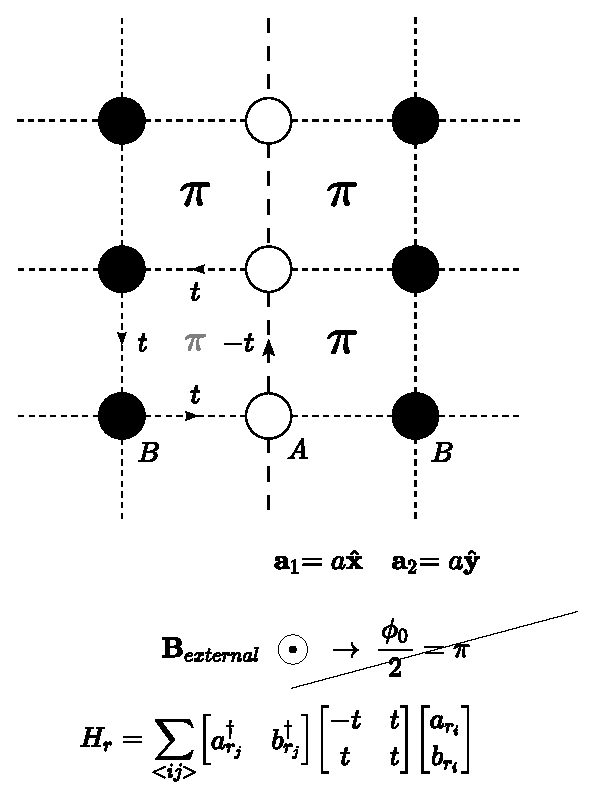
\includegraphics[scale=.7]{sqpi1nn.pdf}
In such a case, which we have depicted, we have the following expression for the Hamiltonian in a second quantized, real-space form:
$$
H_{r}=\sum_{<ij>}
\begin{bmatrix}
a^{\dagger}_{r_j} & b^{\dagger}_{r_j}
\end{bmatrix}
\begin{bmatrix}
-t & t\\
t & t 
\end{bmatrix}
\begin{bmatrix}
a_{r_i} \\ b_{r_i}
\end{bmatrix}
$$
where the sum over $<ij>$ denotes a sum over all pairs $r_i,r_j$ which are nearest neighbors. We thus may expand the above in terms of all points of the lattice $r_i$ and relative displacements $\delta$ such that
$$
\sum_{<ij>} = \sum_{r_i}\sum_{\delta}
$$
with $r_j$ being replaced with $r_i+\delta$ for $\delta$ appropriate for the respective transition. Now, for the $A\rightarrow A$ hoppings, the relevant displacement vectors $\delta$ are $\delta = \pm a\hat{\mathbf{y}}$. Similarly, for $B\rightarrow B$ hoppings we have $\delta = \pm a \hat{\mathbf{y}}$; and then for $A\rightarrow B$ and $B\rightarrow A$  hoppings we have $\delta = \pm a \hat{\mathbf{x}}$.

Now, applying this expansion to our real-space Hamiltonian we get the following:
\begin{align*}
H_{r} =\sum_{r_i}\Bigg( & \sum_{\delta = \pm a \hat{\mathbf{y}}}
\begin{bmatrix}
a^{\dagger}_{r_i+\delta} & b^{\dagger}_{r_i+\delta}
\end{bmatrix}
\begin{bmatrix}
-t & 0\\
0 & t
\end{bmatrix}
\begin{bmatrix}
a_{r_i} \\ b_{r_i}
\end{bmatrix}\\ 
+&
\sum_{\delta = \pm a \hat{\mathbf{x}}}
\begin{bmatrix}
a^{\dagger}_{r_i+\delta} & b^{\dagger}_{r_i+\delta}
\end{bmatrix}
\begin{bmatrix}
0 & t\\
t & 0
\end{bmatrix}
\begin{bmatrix}
a_{r_i} \\ b_{r_i}
\end{bmatrix}\Bigg)
\end{align*}

Now, we may insert the Fourier transform of these creation and annihilation operators:
$$
c^{\dagger}_{r_i} = \frac{1}{\sqrt{N_s}}\sum_j e^{-i\mathbf{q}\cdot\mathbf{r}_i}c_{q}^{\dagger},
$$
$$
c_{r_i} = \frac{1}{\sqrt{N_s}}\sum_q e^{i\mathbf{q}\cdot\mathbf{r}_i}c_{q};
$$
to arrive at the following expression for $H$ in terms of reciprocal lattice vectors (and hence it's form in momentum-space):
\small
\begin{align*}
H_k =& \\
\sum_{k}
\begin{bmatrix}
a^{\dagger}_{k} & b^{\dagger}_{k}
\end{bmatrix}&
\begin{bmatrix}
-t(e^{ik_y a}+e^{-ik_y a}) & t(e^{ik_x a}+e^{-ik_x a})\\
t(e^{ik_x a}+e^{-ik_x a}) & t(e^{ik_y a}+e^{-ik_y a})
\end{bmatrix}
\begin{bmatrix}
a_{k} \\ b_{k}
\end{bmatrix}\\
= &\sum_{k}
\begin{bmatrix}
a^{\dagger}_{k} & b^{\dagger}_{k}
\end{bmatrix}\begin{bmatrix}
-2t\cos(k_y a) & 2t\cos(k_x) a\\
2t\cos(k_x a) & 2t\cos(k_y a)
\end{bmatrix}
\begin{bmatrix}
a_{k} \\ b_{k}
\end{bmatrix}
\end{align*}
\normalsize

From this expression, we may solve for the resulting dispersion relation by diagonalizing the above matrix sandwiched in the product (recoginizing it's role from the general form of the second-quantized Hamiltonian $H=\sum_k \varepsilon(\mathbf{k})c^{\dagger}_kc_k$). This gives the following form (from the 2x2's eigenvalues) of the dispersion:
$$
\varepsilon_{\pm}(\mathbf{k}) = \pm 2t\sqrt{\cos^2(k_y a)+\cos^2(k_x a)}
$$
which has stationary points at the k-space points $\mathbf{k}= (\pm\frac{\pi}{2a},\pm\frac{\pi}{2a})$.

\subsubsection{Dirac Points}
Now, these k-space points behave as Dirac points, in that they have a linear behavior in neighborhoods around them. We now consider, as a specific example, the neighborhood of the point $K=(\pi/2a, \pi/2a)$ by substituting into the dispersion relation the form $k=K+q$. 
\begin{align*}
\varepsilon_{\pm}(\mathbf{q})&=\pm 2t\sqrt{\cos^2\left(\frac{\pi}{2}+q_y a\right)+\cos^2\left(\frac{\pi}{2}+q_x a\right)}\\
& = \pm 2t\sqrt{\sin^2\left(q_y a\right)+\sin^2\left(q_x a\right)}\\
& = \pm 2t\sqrt{(q_y a + ...)^2+(q_x a + ...)^2}\\
& =\pm 2t |\mathbf{q}|a+\mathcal{O}(q^3)
\end{align*}
Hence, the dispersion relation around these points acts linearly in sufficiently small neighborhoods of these points.

\subsection{Second Nearest Neighbor Hopping}
We now consider a second nearest neighbors hopping model, which effectively adds a second sum to the real-space form of our previous (nearest neighbors only) Hamiltonian.
\begin{center}
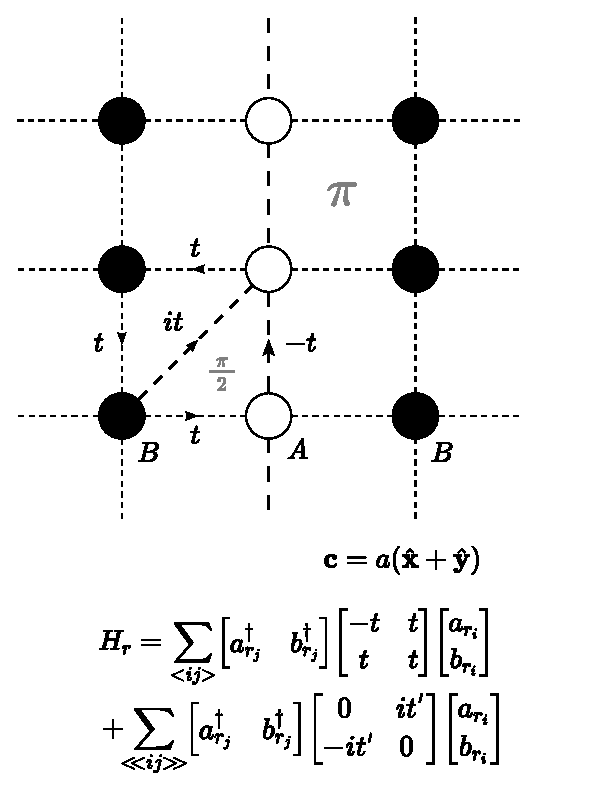
\includegraphics[scale=.7]{sqpi2nn.pdf}
\end{center}
where $\langle\langle ij\rangle\rangle$ denotes the set of all second nearest neighbors only.
\columnbreak

As before, we now expand the sum over nearest neighbors in terms of all real-space lattice vectors. We also expand the sum over second nearest neighbors in similar terms, with the relevant displacement vectors now being $\delta = \pm a (\hat{\mathbf{x}}\pm \hat{\mathbf{y}})$. Note, further, that these second neighbor hoppings only allow for $A\rightarrow B$ and $B\rightarrow A$ site hopping.

Applying all of the above to our real-space Hamiltonian results in the following:
\small
\begin{align*}
H_{r} =\sum_{r_i}&\Bigg(  \sum_{\delta = \pm a \hat{\mathbf{y}}}
\begin{bmatrix}
a^{\dagger}_{r_i+\delta} & b^{\dagger}_{r_i+\delta}
\end{bmatrix}
\begin{bmatrix}
-t & 0\\
0 & t
\end{bmatrix}
\begin{bmatrix}
a_{r_i} \\ b_{r_i}
\end{bmatrix}\\ 
+&
\sum_{\delta = \pm a \hat{\mathbf{x}}}
\begin{bmatrix}
a^{\dagger}_{r_i+\delta} & b^{\dagger}_{r_i+\delta}
\end{bmatrix}
\begin{bmatrix}
0 & t\\
t & 0
\end{bmatrix}
\begin{bmatrix}
a_{r_i} \\ b_{r_i}
\end{bmatrix}\\
+&\sum_{\delta = \pm a (\hat{\mathbf{x}}+\hat{\mathbf{y}})}
\begin{bmatrix}
a^{\dagger}_{r_i+\delta} & b^{\dagger}_{r_i+\delta}
\end{bmatrix}
\begin{bmatrix}
0 & it'\\
-it' & 0
\end{bmatrix}
\begin{bmatrix}
a_{r_i} \\ b_{r_i}
\end{bmatrix}\\
+&\sum_{\delta = \pm a (\hat{\mathbf{x}}-\hat{\mathbf{y}})}
\begin{bmatrix}
a^{\dagger}_{r_i+\delta} & b^{\dagger}_{r_i+\delta}
\end{bmatrix}
\begin{bmatrix}
0 & -it'\\
it' & 0
\end{bmatrix}
\begin{bmatrix}
a_{r_i} \\ b_{r_i}
\end{bmatrix}
\Bigg).
\end{align*}
\normalsize
Again, we now insert the Fourier transform  of the creation and annihilation operators to arrive at an expression of $H$ in terms of momentum-space vectors.\small
\begin{align*}
H_k &= \sum_k \Bigg(  \begin{bmatrix}
a^{\dagger}_{k} & b^{\dagger}_{k}
\end{bmatrix}\begin{bmatrix}
-2t\cos(k_y a) & 2t\cos(k_x) a\\
2t\cos(k_x a) & 2t\cos(k_y a)
\end{bmatrix}
\begin{bmatrix}
a_{k} \\ b_{k}
\end{bmatrix}
\\
+ 2it'&\begin{bmatrix}
a^{\dagger}_{k} & b^{\dagger}_{k}
\end{bmatrix}\begin{bmatrix}
0 & \sin(k_x a +k_ya)\\
-\sin(k_x a -k_ya) & 0
\end{bmatrix}
\begin{bmatrix}
a_{k} \\ b_{k}
\end{bmatrix}
\Bigg)\\
\end{align*}
\normalsize

Now, we solve for the dispersion relation by taking the eigenvalues of the momentum-space form of the Hamiltonian. These eigenvalues yield the dispersion relation:
\small
\begin{align*}
&\varepsilon_{\pm}(\mathbf{k}) = \\
\pm &\sqrt{\left(2t\cos(k_y a)\right)^2+\left(2t\cos(k_x a)\right)^2+\left(4t'\sin(k_xa)\sin(k_ya)\right)^2}
\end{align*}
\normalsize


\section{Honeycomb Lattice}
We now consider a honeycomb lattice (like graphene). 

\subsection{Nearest Neighbor Hopping}
We first consider only first nearest neighbor hopping on the honeycomb.
As before, we consider the real-space honeycomb lattice to be two overlaid Bravais lattices (though here it's overlaid triangular lattices), with one denoted by $A$ sites, and the other $B$ sites, as depicted below.
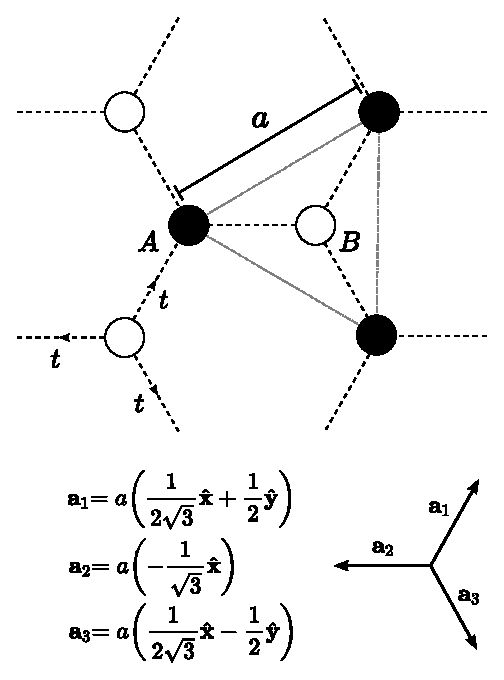
\includegraphics[scale=0.85]{hc1nn.pdf}
Here, nearest neighbor hopping doesn't allow for $A\rightarrow A$ or $B\rightarrow B$ hopping. Thus, we have only off diagonal terms in the real-space Hamiltonian. We also assume an isotropic hopping parameter of $t$ (as before) and hence have a Hamiltonian of the form:
$$
H_r = 
\sum_{<ij>}
\begin{bmatrix}
a^{\dagger}_{r_j} & b^{\dagger}_{r_j}
\end{bmatrix}
\begin{bmatrix}
0& t\\
t & 0
\end{bmatrix}
\begin{bmatrix}
a_{r_i} \\ b_{r_i}
\end{bmatrix}
$$
Expanding the nearest neighbor sum in terms of the lattice vectors and the relevant displacement vectors for $A\rightarrow
B$  and $B\rightarrow A$ hopping, which are $-a_1,-a_2,-a_3$ and $a_1,a_2,a_3$ respectively, we then get the following expanded form of the real-space Hamiltonian:
\begin{align*}
H_r &= 
\sum_{r_i}\sum_{\delta}^{a_1,a_2,a_3}
\begin{bmatrix}
a^{\dagger}_{r_i+\delta} & b^{\dagger}_{r_i-\delta}
\end{bmatrix}
\begin{bmatrix}
0& -t\\
-t & 0
\end{bmatrix}
\begin{bmatrix}
a_{r_i} \\ b_{r_i}
\end{bmatrix}\\
\end{align*}
Again, substituting in the Fourier transform of the creation and annihilation operators, we get the following form of the Hamiltonian in momentum-space:
\small
\hspace{-1.5cm}
\begin{align*}
H_k = 
-t\sum_{k}
\begin{bmatrix}
a^{\dagger}_{k} &b^{\dagger}_{k}
\end{bmatrix} 
\quad\quad\quad\quad\quad\quad\quad\quad\quad
\quad\quad\quad\quad\quad\quad
\\ \times
\begin{bmatrix}
0& e^{ik\cdot a_1}+e^{ik\cdot a_2}+e^{ik\cdot a_3}\\
e^{-ik\cdot a_1}+e^{-ik\cdot a_2}+e^{-ik\cdot a_3} & 0
\end{bmatrix} \\
\quad\quad\quad\quad\quad\quad
\times\begin{bmatrix}
a_{k} \\ b_{k}
\end{bmatrix}\\
\end{align*}
\normalsize
Diagonalizing this results in the eigenvalues, giving the dispersion relation:
$$
\varepsilon_{\pm}(\mathbf{k})=\pm t\ |e^{ik\cdot a_1}+e^{ik\cdot a_2}+e^{ik\cdot a_3}|
$$
which has minimums at $\mathbf{k}=A,B$ where $A,B$ denotes any of the honeycomb sites.

\subsubsection{Dirac Points}
These minimum points of the dispersion again act as Dirac points, as evidenced by their linear behavior in neighborhoods around such points.

This may been seen in a Taylor expansion around an arbitrary $K$ point of the form $\mathbf{k}=\mathbf{K}+\mathbf{q}$:
\begin{align*}
\varepsilon_{\pm}(\mathbf{q})&=\pm t\ |e^{i(\mathbf{K}+\mathbf{q})\cdot a_1}+e^{i(\mathbf{K}+\mathbf{q})\cdot a_2}+e^{i(\mathbf{K}+\mathbf{q})\cdot a_3}|\\
& = \pm t |(1+i(\mathbf{K}+\mathbf{q})\cdot \mathbf{a_1}+...)\\
&\quad\ \ +(1+i(\mathbf{K}+\mathbf{q})\cdot \mathbf{a_2}+...)\\
&\quad\ \ +(1+i(\mathbf{K}+\mathbf{q})\cdot \mathbf{a_3}+...)|\\
\end{align*}
Now, consider the specific $\mathbf{K}= \frac{}{}\left(\right)$


\subsection{Second Nearest Neighbor Hopping}
Now we consider second nearest neighbor hopping on the honeycomb lattice, in addition to the first nearest neighbor hopping just considered. 

Since second nearest neighbors are always of the same underlying Bravais lattice, the relevant terms are those of $A\rightarrow A$ and $B\rightarrow B$ hopping. Hence, these second nearest neighbors only contribute diagonal terms to the Hamiltonian. 

We use a model for these hoppings that is spin-dependent and of the form:
$$
H_{SOC}^{2^{nd}-nn} = i\lambda\sum_{\langle\langle ij \rangle\rangle} \sum_{\alpha\beta}^{\uparrow \downarrow} c^{\dagger}_{r_i \alpha}\left[ \hat{\mathbf{e}}_{ij}\cdot \hat{\mathbf{s}} \right]_{\alpha\beta}c_{r_j \beta}
$$ 
where $\hat{\mathbf{e}}_{ij}$ represents the direction of the turn taken in getting to next nearest neighbor (assuming it travels along the honeycomb lattice); $\hat{\mathbf{s}}$ represents the Pauli matrix vector (which acts on the spin space); and the second indices of the creation and annihilation operators ($\alpha,\beta$) represent the spin state of the particles (up or down along the axis perpendicular the plane).

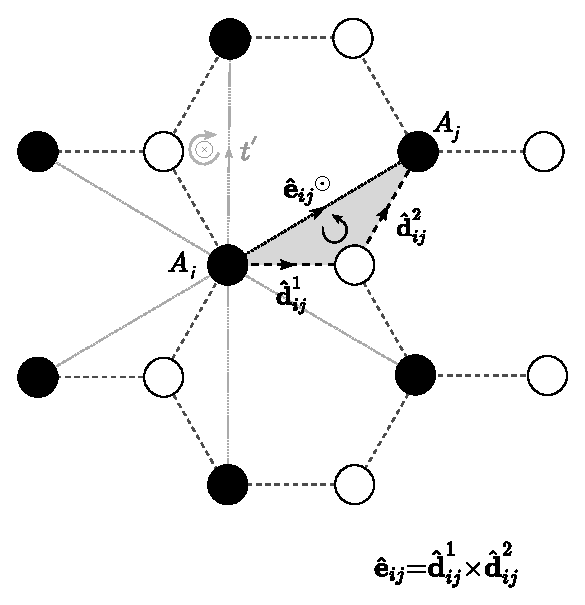
\includegraphics[scale=0.7]{hc2nn.pdf}
\noindent
Combining this with the first neighbor hopping real-space Hamiltonian yields the following:
\begin{align*}
H_r &= 
\sum_{<ij>}\sum_{\alpha}^{\uparrow \downarrow}
\begin{bmatrix}
a^{\dagger}_{r_j\alpha} & b^{\dagger}_{r_j\alpha}
\end{bmatrix}
\begin{bmatrix}
0& t\\
t & 0
\end{bmatrix}
\begin{bmatrix}
a_{r_i\alpha} \\ b_{r_i\alpha}
\end{bmatrix}\\
& +i\lambda\sum_{\langle\langle ij \rangle\rangle}\sum_{\alpha\beta}^{\uparrow \downarrow}\sum_{c}^{a,b} c^{\dagger}_{r_j \alpha}\left[ \hat{\mathbf{e}}_{ij}\cdot \hat{\mathbf{s}} \right]_{\alpha\beta}c_{r_i \beta}\\
\end{align*}
We now expand the sum over spin indices as tensors in the product overall, after defining a convenient creation and annihilation vector below.
$$
\vec{a}^{\dagger}_{r_i} = \begin{bmatrix}
a_{r_i\uparrow}^{\dagger } & a_{r_i\downarrow}^{\dagger }
& b_{r_i\uparrow}^{\dagger } & b_{r_i\downarrow}^{\dagger }
\end{bmatrix}
$$

\begin{align*}
H_r &= 
\sum_{<ij>}
\vec{a}^{\dagger}_{r_j}\left(
\begin{bmatrix}
0& t\\
t & 0
\end{bmatrix}\otimes\mathbb{I}_{spin}\right)
\vec{a}_{r_i}\\
& +i\lambda\sum_{\langle\langle ij \rangle\rangle} \vec{a}^{\dagger}_{r_j}\left(\mathbb{I}_{orb}\otimes\left[ \hat{\mathbf{e}}_{ij}\cdot \hat{\mathbf{s}} \right]\right)\vec{a}_{r_i}\\
\end{align*}

Note that, while both the $A$ and $B$ triangular lattices share the same Bravais lattice vectors, the orientation or handedness of the corresponding unit vectors $\hat{\mathbf{e}}_{ij}$ are reversed between the two sub lattices (hence it's second neighbors term's action as a Pauli Z matrix on the orbital subspace).

Also note that, since the unit vector $\hat{\mathbf{e}}_{ij}=\pm \hat{\mathbf{z}}$ due to the planar nature of the lattice, $ \hat{\mathbf{e}}_{ij}\cdot \hat{\mathbf{s}}$ must always be either $\pm \sigma^z$ (where $\sigma^z$ acts on the spin space and identity on the orbital space). Each site on one of the triangular Bravais lattice's has six second nearest neighbors, with three of $\hat{\mathbf{e}}_{ij} = +\hat{\mathbf{z}}$ and three with $\hat{\mathbf{e}}_{ij} =-\hat{\mathbf{z}}$. For the $A$ lattice the set of positive Z spin operators correspond to the lattice vectors $\delta_j^+=\mathbf{A}_1,-\mathbf{A}_2,-\mathbf{A}_3$, with those corresponding to negative $\hat{\mathbf{e}}_{ij}$ being $\delta_j^-=-\mathbf{A}_1,\mathbf{A}_2,\mathbf{A}_3$. For the $B$ sublattice the correspondence is reversed.


We now expand the real-space Hamiltonian in terms of displacement vectors, as before. 
\begin{align*}
H_r &= 
\sum_{r_i}\sum_{\delta}
\vec{a}^{\dagger}_{r_i+\delta}\left(
\begin{bmatrix}
0& t\\
t & 0
\end{bmatrix}\otimes\mathbb{I}\right)
\vec{a}_{r_i}\\
& +i\lambda\sum_{r_i} \sum_{j=1}^3\vec{a}^{\dagger}_{r_i+\delta_j^+}\left(\mathbb{I}\otimes\sigma^z \right)\vec{a}_{r_i}\\
& -i\lambda\sum_{r_i} \sum_{j=1}^3\vec{a}^{\dagger}_{r_i+\delta_j^-}\left(\mathbb{I}\otimes\sigma^z \right)\vec{a}_{r_i}\\
\end{align*}
\begin{center}
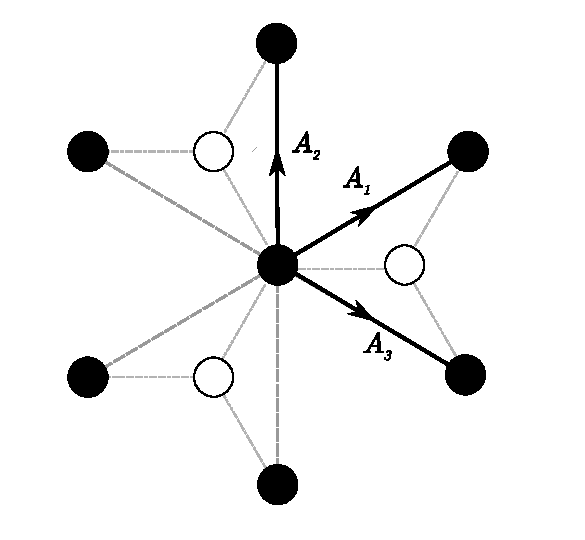
\includegraphics[scale=0.65]{hc2nnA.pdf}
\end{center}
\noindent
And now expand in terms of the Fourier transform of $\vec{a}_{r_i}$ to arrive at a form in $k$-space:
\begin{align*}
\Rightarrow \ \ H_k & = \sum_{k}
\vec{a}^{\dagger}_{k}\left(
\begin{bmatrix}
0& f_1(\mathbf{k})\\
f^*_1(\mathbf{k}) & 0
\end{bmatrix}\otimes\mathbb{I}\right)
\vec{a}_{k}\\
& +\sum_{k} \vec{a}^{\dagger}_{k}d_5(\mathbf{k})\left(\sigma^z\otimes\sigma^z \right)\vec{a}_{k}\\
& = \sum_{k}
\vec{a}^{\dagger}_{k}\Big(d_1(\mathbf{k})
(\sigma_x\otimes\mathbb{I})+d_2(\mathbf{k})
(\sigma_y\otimes\mathbb{I})\\
&\quad\quad\quad\quad\quad\quad
\quad\quad\quad\quad\quad
 + d_5(\mathbf{k})\sigma^z\otimes\sigma^z \Big)\vec{a}_{k}\\
\end{align*}

\vspace{-1cm}

\begin{center}
where 
$$f_1(\mathbf{k})=t(e^{ik\cdot a_1}+e^{ik\cdot a_2}+e^{ik\cdot a_3})=d_1(\mathbf{k})+id_2(\mathbf{k})$$
(from the previous section) and 
$$d_5(\mathbf{k})=2\lambda\big[\sin(\mathbf{k}\cdot\mathbf{A}_1)-\sin(\mathbf{k}\cdot\mathbf{A}_2)-\sin(\mathbf{k}\cdot\mathbf{A}_3)\big]$$
\end{center}
Now, applying the formula for the band energy from \cite{aa} from equation (4.8):
$$
\varepsilon(\mathbf{k})_{\pm}= d_0(\mathbf{k})\pm \sqrt{\sum_{a=1}^5d_a(\mathbf{k})^2}
$$
we can easily solve for the dispersion relation in terms of our form of $H_k$ to arrive at:
\footnotesize	
\begin{align*}
&\varepsilon(\mathbf{k})_{\pm}=\pm\\ &\sqrt{|f_1(\mathbf{k})|^2+4\lambda^2\big[\sin(\mathbf{k}\cdot\mathbf{A}_1)-\sin(\mathbf{k}\cdot\mathbf{A}_2)-\sin(\mathbf{k}\cdot\mathbf{A}_3)\big]^2}
\end{align*}
\normalsize
which is non-degenerate everywhere, with a minimum gap of $\lambda$ at the previously gapless (in the first neighbors model) $K,K'$ points.

\subsubsection{Time-Reversal Points and $\mathbb{Z}_2$ Invariant}
The four time-reversal symmetric points $\Gamma_ij$ for the honeycomb lattice are 
$\Gamma_{n_1 n_2}=n_1 \mathbf{\gamma}_1+n_2\mathbf{\gamma}_2$ with $n_1,n_2 = 0,1$. Then, from equation (4.10) of \cite{aa}, we have:
$$
\delta_{n_1 n_2} = -\text{sgn}\left[d_1(\Gamma_{n_1 n_2})\right]
$$
and from (2.10) in the same paper we have:
$$
(-1)^{\nu}=\prod_{n_1,n_2}^{0,1}\delta_{n_1 n_2}
$$
for the $\mathbb{Z}_2$ invariant.
From our form of the $k$-space Hamiltonian we have the expression for $d_1(\mathbf{k})$:
$$
d_1(\mathbf{k})= t\big(\cos(\mathbf{k}\cdot\mathbf{a}_1)+\cos(\mathbf{k}\cdot\mathbf{a}_2)+\cos(\mathbf{k}\cdot\mathbf{a}_3)\big)
$$
At $\mathbf{k}=\Gamma_{00}=0$, this $d_1(\mathbf{k})$ clearly has a positive value, as well as at $\mathbf{k}=\Gamma_{01},\Gamma_{10}$ since at these points we have

At $\mathbf{k}=\Gamma_{11}$, however, $d_1(\mathbf{k})$ is negative.
\begin{center}
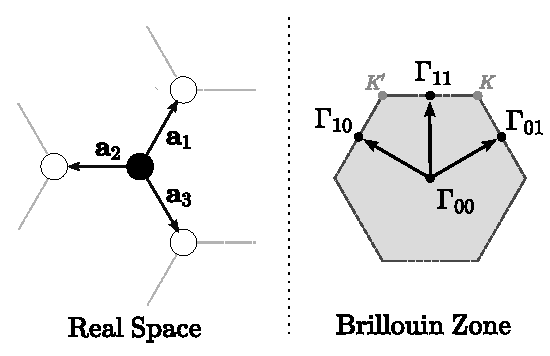
\includegraphics[scale=0.8]{gampts.pdf} 
\end{center}
Hence, we have an odd $\nu$ for graphene in this model, which indicates such a model would behave as a quantum spin Hall topological insulator.
\end{multicols}

\begin{thebibliography}{2}

\bibitem{aa} Liang Fu and C. L. Kane, Topological insulators with inversion symmetry, PHYSICAL REVIEW B 76, 045302 (2007)
\end{thebibliography}
\end{document}
